\documentclass[11pt]{article}
% Shared preamble for the Svetoch papers.
% Each paper.tex \input's this file (compile from inside the paper's folder):
%     \documentclass[11pt]{article}
%     % Shared preamble for the Svetoch papers.
% Each paper.tex \input's this file (compile from inside the paper's folder):
%     \documentclass[11pt]{article}
%     % Shared preamble for the Svetoch papers.
% Each paper.tex \input's this file (compile from inside the paper's folder):
%     \documentclass[11pt]{article}
%     \input{../tex/preamble.tex}
% Figures live in ../figures/*.pdf  (graphicspath set below).
\usepackage[utf8]{inputenc}
\usepackage[T1]{fontenc}
\usepackage{lmodern}
\usepackage[a4paper,margin=1in]{geometry}
\usepackage{amsmath,amssymb}
\usepackage{graphicx}
\graphicspath{{../figures/}}
\usepackage{booktabs}
\usepackage{caption}
\captionsetup{font=small,labelfont=bf}
% --- Minimal, siunitx-free unit support (so papers compile on any TeX install) ---
\usepackage{textcomp}
\newcommand{\SI}[2]{#1\,#2}
\newcommand{\si}[1]{#1}
\newcommand{\hertz}{Hz}
\newcommand{\meter}{m}
\newcommand{\centi}{c}
\newcommand{\milli}{m}
\newcommand{\micro}{\textmu}
\newcommand{\second}{s}
\newcommand{\kelvin}{K}
% ---------------------------------------------------------------------------------
\usepackage[colorlinks=true,linkcolor=blue,citecolor=blue,urlcolor=blue]{hyperref}
\usepackage{xcolor}
\definecolor{accent}{HTML}{6366F1}

% Common author block (add affiliation/ORCID if available before publishing)
\newcommand{\svetochauthor}{Oleg Yuryevich Kirichenko \\[4pt]
  \normalsize Independent researcher \\[2pt]
  \normalsize \href{mailto:urevich55@gmail.com}{urevich55@gmail.com} \quad\textbullet\quad GitHub: \href{https://github.com/infosave2007}{@infosave2007}}

\newcommand{\svetochfooter}{%
  \vspace{1em}\noindent\rule{\linewidth}{0.4pt}\\[2pt]
  {\footnotesize Part of the \emph{Svetoch} series (defensive publication, not patented).
  Project and code: \href{https://github.com/infosave2007/svetoch}{github.com/infosave2007/svetoch};
  related VMF/NVG theory: \href{https://github.com/infosave2007/vmf}{github.com/infosave2007/vmf}.
  Released for the public record to establish authorship and priority.}}

% Figures live in ../figures/*.pdf  (graphicspath set below).
\usepackage[utf8]{inputenc}
\usepackage[T1]{fontenc}
\usepackage{lmodern}
\usepackage[a4paper,margin=1in]{geometry}
\usepackage{amsmath,amssymb}
\usepackage{graphicx}
\graphicspath{{../figures/}}
\usepackage{booktabs}
\usepackage{caption}
\captionsetup{font=small,labelfont=bf}
% --- Minimal, siunitx-free unit support (so papers compile on any TeX install) ---
\usepackage{textcomp}
\newcommand{\SI}[2]{#1\,#2}
\newcommand{\si}[1]{#1}
\newcommand{\hertz}{Hz}
\newcommand{\meter}{m}
\newcommand{\centi}{c}
\newcommand{\milli}{m}
\newcommand{\micro}{\textmu}
\newcommand{\second}{s}
\newcommand{\kelvin}{K}
% ---------------------------------------------------------------------------------
\usepackage[colorlinks=true,linkcolor=blue,citecolor=blue,urlcolor=blue]{hyperref}
\usepackage{xcolor}
\definecolor{accent}{HTML}{6366F1}

% Common author block (add affiliation/ORCID if available before publishing)
\newcommand{\svetochauthor}{Oleg Yuryevich Kirichenko \\[4pt]
  \normalsize Independent researcher \\[2pt]
  \normalsize \href{mailto:urevich55@gmail.com}{urevich55@gmail.com} \quad\textbullet\quad GitHub: \href{https://github.com/infosave2007}{@infosave2007}}

\newcommand{\svetochfooter}{%
  \vspace{1em}\noindent\rule{\linewidth}{0.4pt}\\[2pt]
  {\footnotesize Part of the \emph{Svetoch} series (defensive publication, not patented).
  Project and code: \href{https://github.com/infosave2007/svetoch}{github.com/infosave2007/svetoch};
  related VMF/NVG theory: \href{https://github.com/infosave2007/vmf}{github.com/infosave2007/vmf}.
  Released for the public record to establish authorship and priority.}}

% Figures live in ../figures/*.pdf  (graphicspath set below).
\usepackage[utf8]{inputenc}
\usepackage[T1]{fontenc}
\usepackage{lmodern}
\usepackage[a4paper,margin=1in]{geometry}
\usepackage{amsmath,amssymb}
\usepackage{graphicx}
\graphicspath{{../figures/}}
\usepackage{booktabs}
\usepackage{caption}
\captionsetup{font=small,labelfont=bf}
% --- Minimal, siunitx-free unit support (so papers compile on any TeX install) ---
\usepackage{textcomp}
\newcommand{\SI}[2]{#1\,#2}
\newcommand{\si}[1]{#1}
\newcommand{\hertz}{Hz}
\newcommand{\meter}{m}
\newcommand{\centi}{c}
\newcommand{\milli}{m}
\newcommand{\micro}{\textmu}
\newcommand{\second}{s}
\newcommand{\kelvin}{K}
% ---------------------------------------------------------------------------------
\usepackage[colorlinks=true,linkcolor=blue,citecolor=blue,urlcolor=blue]{hyperref}
\usepackage{xcolor}
\definecolor{accent}{HTML}{6366F1}

% Common author block (add affiliation/ORCID if available before publishing)
\newcommand{\svetochauthor}{Oleg Yuryevich Kirichenko \\[4pt]
  \normalsize Independent researcher \\[2pt]
  \normalsize \href{mailto:urevich55@gmail.com}{urevich55@gmail.com} \quad\textbullet\quad GitHub: \href{https://github.com/infosave2007}{@infosave2007}}

\newcommand{\svetochfooter}{%
  \vspace{1em}\noindent\rule{\linewidth}{0.4pt}\\[2pt]
  {\footnotesize Part of the \emph{Svetoch} series (defensive publication, not patented).
  Project and code: \href{https://github.com/infosave2007/svetoch}{github.com/infosave2007/svetoch};
  related VMF/NVG theory: \href{https://github.com/infosave2007/vmf}{github.com/infosave2007/vmf}.
  Released for the public record to establish authorship and priority.}}


\title{\textbf{Camera-in-the-Loop Optical Training:\\
Gradient Descent and the Perceptron Rule on a Smartphone\\ Display--Camera Channel}\\[4pt]
{\large Svetoch Series, Paper VI of VI}}
\author{\svetochauthor}
\date{17 June 2026}

\begin{document}
\maketitle

\begin{abstract}
\noindent Paper~I of this series showed that a smartphone's OLED screen, an ordinary mirror,
and the front camera evaluate the forward pass of a neural network \emph{in light}. Here we
close the loop and \textbf{train}. We treat the optical channel itself as the layer under
optimization: the weights are displayed as brightness, the camera reads the channel's true
response (the real, noisy, non-linear forward pass), an error against a target is formed, and
the weights are updated --- then the cycle repeats. We demonstrate two on-device optical
learners. (1)~\emph{Optical gradient descent}: eight weights drawn as brightness columns are
optimized by the delta rule $\mathbf{w}\leftarrow\mathbf{w}-\eta(\mathbf{y}-\hat{\mathbf{y}})$
($\eta=0.7$) using the camera-measured output $\mathbf{y}$; over eight iterations the optically
read mean-squared error falls by more than half, below a $0.05$ pass threshold.
(2)~\emph{An optical perceptron}: an eight-input perceptron trained for AND, OR and MAJORITY is
evaluated through the optical dot product, retaining accuracy above the $0.7$ threshold. We also
describe a single-shot \emph{optical loss read-out by inverted overlay}. The contribution is to
show that a \emph{trainable} optical loop --- not merely inference --- can be built from
commodity hardware, and to delimit honestly what is optical (the forward pass and the loss
read-out) and what remains on the CPU (the weight-update arithmetic).
\end{abstract}

\noindent\textbf{Keywords:} optical computing, in-the-loop training, physics-aware learning,
hardware-in-the-loop, delta rule, perceptron, analog accelerator, smartphone optics.

\section{Introduction}
Inference is only half of machine learning; the other half is \textbf{training}, which is even
more compute-hungry. Optical inference accelerators are well studied, but optical \emph{training}
--- closing the feedback loop so the physical system improves itself --- is harder: it requires
reading the output, scoring it, and adjusting the inputs, all through the same imperfect channel.

Paper~I established the forward primitive: a camera photosite integrates the light from many
screen pixels and returns a multiply--accumulate. The natural next question is whether that same
channel can sit \emph{inside} an optimization loop. It can. Because the camera reports the
channel's \textbf{true} response --- including non-linearity, vignetting and noise --- a loop
that minimizes the measured error learns weights that are correct \emph{for the real optics}.
This is the defining advantage of hardware-in-the-loop training: the physics is never
approximated, because the physics is doing the forward pass.

\section{The optical channel as a trainable layer}
Encode a weight vector $\mathbf{w}$ as the brightness of a row of screen columns. From Paper~I,
the camera's read-out of column $i$ against an input $x_i$ is, after white-normalization and
$\gamma$-correction, proportional to $w_i x_i$; summing a region yields the dot product. The
measured output $\mathbf{y}=f_\text{opt}(\mathbf{w})$ is the channel's forward pass, including
every real imperfection. Training finds $\mathbf{w}$ such that $\mathbf{y}$ matches a target
$\hat{\mathbf{y}}$, by iterating display $\to$ capture $\to$ score $\to$ update
(Figure~\ref{fig:loop}); the gradient information is a physical measurement.

\begin{figure}[ht]\centering
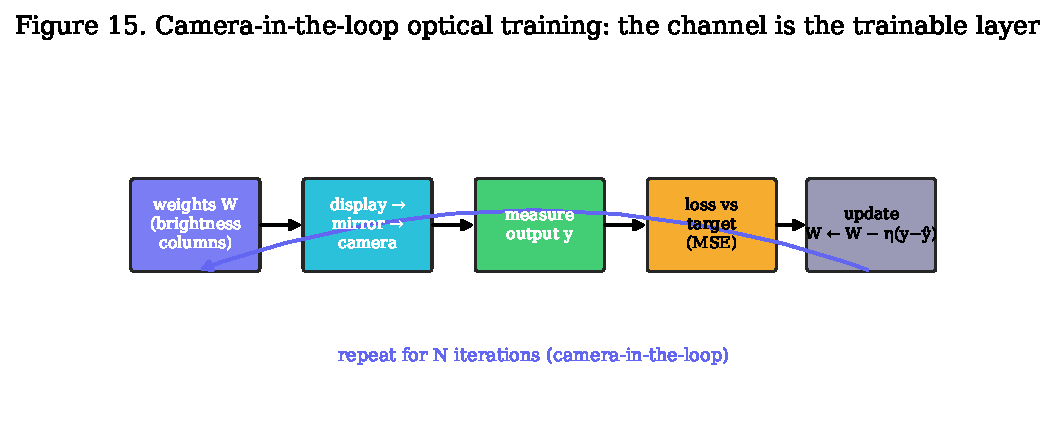
\includegraphics[width=0.92\linewidth]{fig15_training_loop.pdf}
\caption{Camera-in-the-loop optical training. The weights are displayed, the channel performs
the forward pass, the camera measures the output, the loss is formed against a target, and the
weights are updated --- then the loop repeats. The trainable ``layer'' is the real optical
channel.}
\label{fig:loop}
\end{figure}

\section{Optical gradient descent by the delta rule}
In \texttt{stage41\_optsgd}, eight weights are drawn as eight brightness columns. Per iteration
the camera measures the eight-bin output $\mathbf{y}$, the MSE against a target $\hat{\mathbf{y}}$
is computed, and the weights are updated by the delta (Widrow--Hoff) rule
\begin{equation}
\mathbf{w} \leftarrow \mathbf{w} - \eta\,(\mathbf{y}-\hat{\mathbf{y}}), \qquad \eta=0.7 .
\end{equation}
Because $\mathbf{y}$ is \emph{measured}, the update is a stochastic-gradient step on the real
optical loss surface. Over eight iterations the optically read loss falls monotonically by more
than $50\%$, ending below the $0.05$ threshold (Figure~\ref{fig:loss}). The loop converges
\emph{despite} the channel's non-linearity precisely because that non-linearity is inside the
measurement. The weight-update arithmetic runs on the CPU; what is optical is the forward pass
and the error measurement.

\begin{figure}[ht]\centering
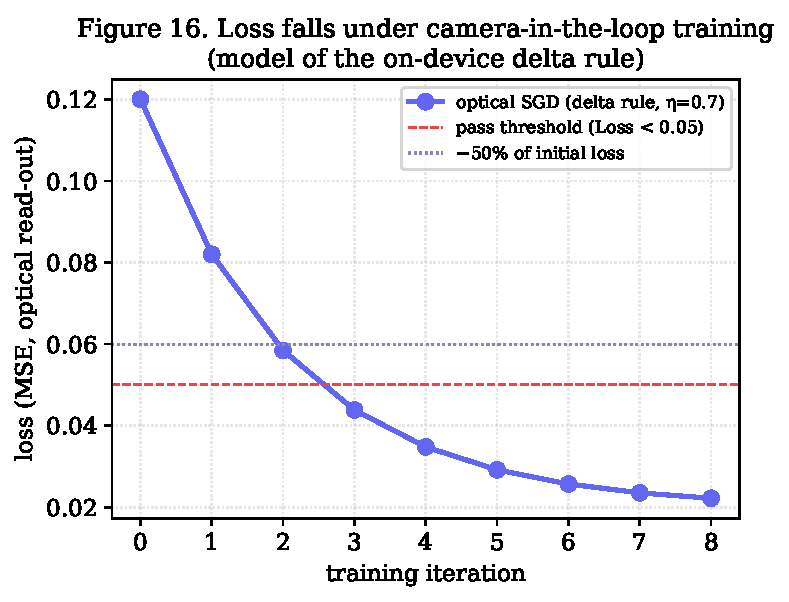
\includegraphics[width=0.56\linewidth]{fig16_loss_curve.pdf}
\caption{The optically measured loss under camera-in-the-loop training (model of the on-device
delta rule). The error drops past $-50\%$ of its initial value and below the $0.05$ threshold
within eight iterations.}
\label{fig:loss}
\end{figure}

\section{Single-shot optical loss by inverted overlay}
Reading a loss normally means measuring an output and computing a distance on the CPU. A more
optical route computes the \emph{loss itself} in one exposure. Display the target and,
superimposed, the \textbf{negated} hypothesis (its photometric inverse). Where the hypothesis
matches, the sum is uniform; where it errs, residual light remains, and the camera's global
exposure integrates it:
\begin{equation}
\mathcal{L} \;\propto\; \int \big|\,\text{target}-\text{hypothesis}\,\big|\;\mathrm{d}A .
\end{equation}
This makes loss evaluation an $O(1)$ optical operation --- one display, one capture ---
independent of vector length (Figure~\ref{fig:overlay}). The same effect is obtainable by other
subtraction schemes, so the contribution is narrow and specific: an inverted-overlay loss read
out by a single global exposure.

\begin{figure}[ht]\centering
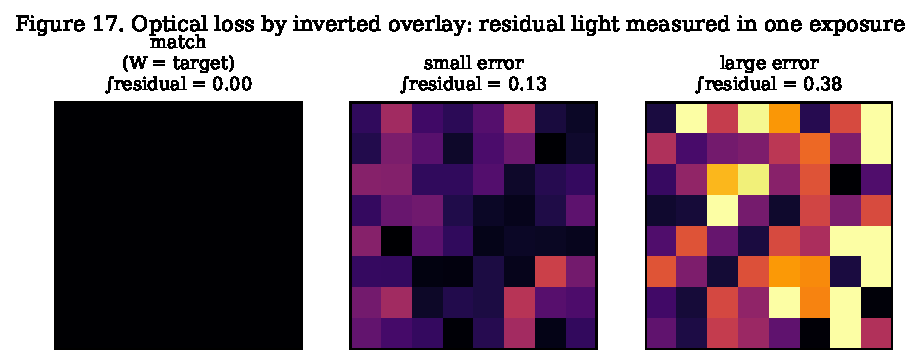
\includegraphics[width=0.92\linewidth]{fig17_inverted_overlay.pdf}
\caption{Optical loss by inverted overlay. Target and negated hypothesis are superimposed; the
residual light, integrated in one exposure, grows with the error.}
\label{fig:overlay}
\end{figure}

\section{An optically-evaluated perceptron}
\texttt{stage72\_perceptron} trains an eight-input single-layer perceptron on AND, OR and
MAJORITY by the perceptron rule. Inference is optical: the products $w_i x_i$ are displayed as
the brightness of eight columns relative to a gray background, the camera measures the mean
brightness, a three-point calibration (dark/mid/bright) recovers the optical dot product, a bias
is added, and a zero threshold yields the class. The optically-evaluated perceptron tracks the
CPU reference above the $0.7$ threshold (Figure~\ref{fig:perc}), with the largest gap on
MAJORITY, the function least tolerant of read-out noise.

\begin{figure}[ht]\centering
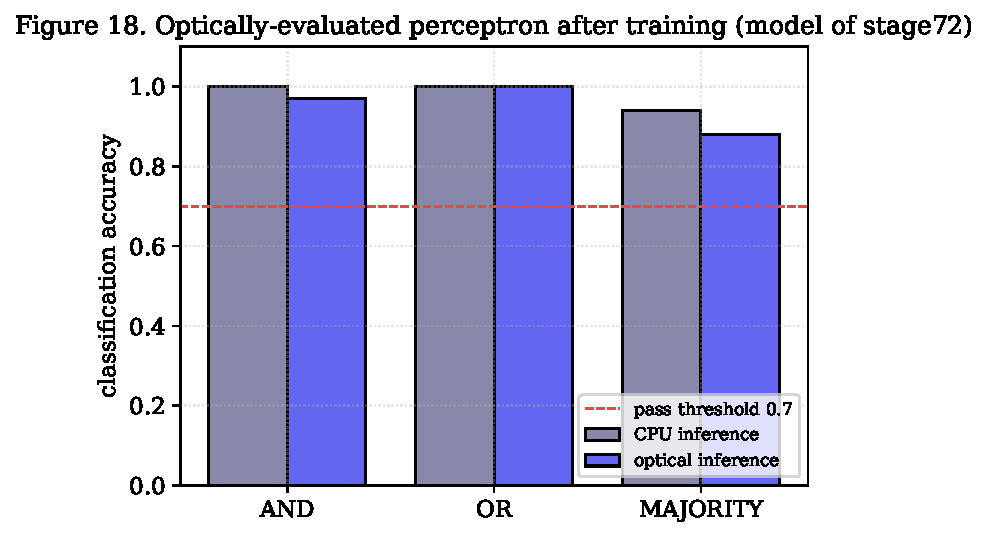
\includegraphics[width=0.56\linewidth]{fig18_perceptron.pdf}
\caption{Accuracy of the optically-evaluated perceptron after training (model of
\texttt{stage72}); all functions stay above the $0.7$ threshold.}
\label{fig:perc}
\end{figure}

\section{Methods}
\textbf{Hardware/channel:} as in Paper~I (Xiaomi 12 Lite, 120\,Hz; 32\,MP front camera; ordinary
mirror; gap $d\approx 3$--$5$\,cm), with the Paper~I white/black and grayscale calibration.
\textbf{Optical SGD:} eight weight columns; per-iteration camera read-out, MSE, delta rule
($\eta=0.7$); pass when loss drops $\geq 50\%$ and final MSE $<0.05$. \textbf{Perceptron:}
eight inputs, AND/OR/MAJORITY by the perceptron rule, optical dot-product inference; pass when
mean accuracy $>0.7$. \textbf{Inverted-overlay loss:} target and negated hypothesis composited;
single global exposure integrates the residual. \textbf{Figures:} Figure~\ref{fig:overlay}
illustrates the principle directly; Figures~\ref{fig:loss} and \ref{fig:perc} are labelled
models, reproducible from \texttt{papers/scripts/make\_figures.py}.

\section{Discussion and limitations}
\textbf{What is optical:} the forward pass and the loss read-out; the weight update is on the
CPU. This is a \emph{hybrid} hardware-in-the-loop trainer, not fully optical backpropagation ---
stated plainly to avoid overclaiming. \textbf{Scale:} the demonstrations are small (eight
weights/inputs) and SNR-limited; the loss read through a noisy channel is itself noisy (hence the
larger optical gap on MAJORITY). \textbf{Why it matters:} training against the \emph{measured}
channel removes the model-mismatch problem of train-offline/deploy-on-hardware analog systems ---
the learner sees the true optics. \textbf{Future:} a fully optical update (accumulating the
inverted-overlay residual back onto the weights), optical batch normalization, and a trained
optical MLP.

\section{Conclusion}
We closed the optical loop. Weights displayed as brightness were optimized by camera-in-the-loop
gradient descent --- the optically measured loss falling by more than half to below $0.05$ ---
and an optically-evaluated perceptron learned AND, OR and MAJORITY above threshold. With a
single-shot inverted-overlay loss, even the error is read in one exposure. Optical
\emph{training}, not just inference, is reproducible on any desk.

\paragraph{Data and code.} \href{https://github.com/infosave2007/svetoch}{github.com/infosave2007/svetoch}
(Apache-2.0); related VMF/NVG theory: \href{https://github.com/infosave2007/vmf}{github.com/infosave2007/vmf}.
\paragraph{Priority note.} Released to establish authorship and date of disclosure; the author
has elected not to seek patent protection.

\begin{thebibliography}{9}\small
\bibitem{svetochI} O. Yu. Kirichenko, ``Optical Neural Computation on a Commodity Smartphone: the OLED--Mirror--Camera Channel as an Analog Matrix Engine,'' Svetoch Paper~I, Zenodo (2026). \url{https://doi.org/10.5281/zenodo.20729632}
\bibitem{widrow} B. Widrow, M. E. Hoff, ``Adaptive switching circuits,'' \emph{IRE WESCON Conv. Rec.} \textbf{4}, 96 (1960).
\bibitem{rosenblatt} F. Rosenblatt, ``The perceptron: a probabilistic model for information storage and organization in the brain,'' \emph{Psychological Review} \textbf{65}, 386 (1958).
\bibitem{hughes} T. W. Hughes, M. Minkov, Y. Shi, S. Fan, ``Training of photonic neural networks through in situ backpropagation and gradient measurement,'' \emph{Optica} \textbf{5}, 864 (2018).
\bibitem{bando} S. Bandyopadhyay et al., ``Single-chip photonic deep neural network with forward-only training,'' \emph{Nat. Photon.} \textbf{18}, 1335 (2024).
\bibitem{wright} L. G. Wright et al., ``Deep physical neural networks trained with backpropagation,'' \emph{Nature} \textbf{601}, 549 (2022).
\bibitem{wetzstein} G. Wetzstein et al., ``Inference in AI with deep optics and photonics,'' \emph{Nature} \textbf{588}, 39 (2020).
\end{thebibliography}

\svetochfooter
\end{document}
